% !TEX root = ./stellar_notes.tex

\chapter{Stellar Pulsations}\label{s.pulsations}

In this chapter, we'll linearize the perturbed continuity and momentum equations and solve for the frequencies of the normal modes for a star.

\section{Adiabatic, radial pulsations}\label{s.adiabatic-radial}
Imagine that we perturb our fluid in some way.
As described in section \ref{s.convection-second-look}, we can describe the \emph{Eulerian} perturbation in some fluid property $f$:
\begin{equation}
  \Delta f \equiv f(\vr,t)-f_{0}(\vr,t),
\end{equation}
where the subscript ``0'' denotes the unperturbed quantity. Said another way, $\Delta f$ describes the change, under our perturbation, in some property of the fluid at a fixed location.
\begin{marginfigure}
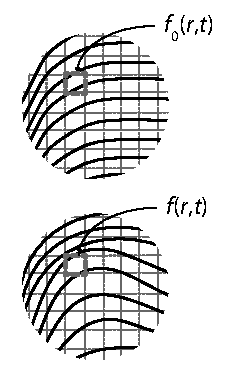
\includegraphics[width=\linewidth]{eulerian}
\caption{\label{f.eulerian-grid} An Eulerian perturbation: we compare quantities at corresponding locations.}
\end{marginfigure}

We may also describe our perturbation as a \emph{Lagrangian} one, where we compare the same fluid element in both the perturbed and unperturbed systems:
\begin{equation}
 \delta f \equiv f(\vr,t) - f_{0}(\vr_{0},t).
\end{equation}
Under a Lagrangian perturbation the fluid element in the perturbed system in general has a different position $\vr$ than in the unperturbed system, $\vr_{0}$.
\begin{marginfigure}
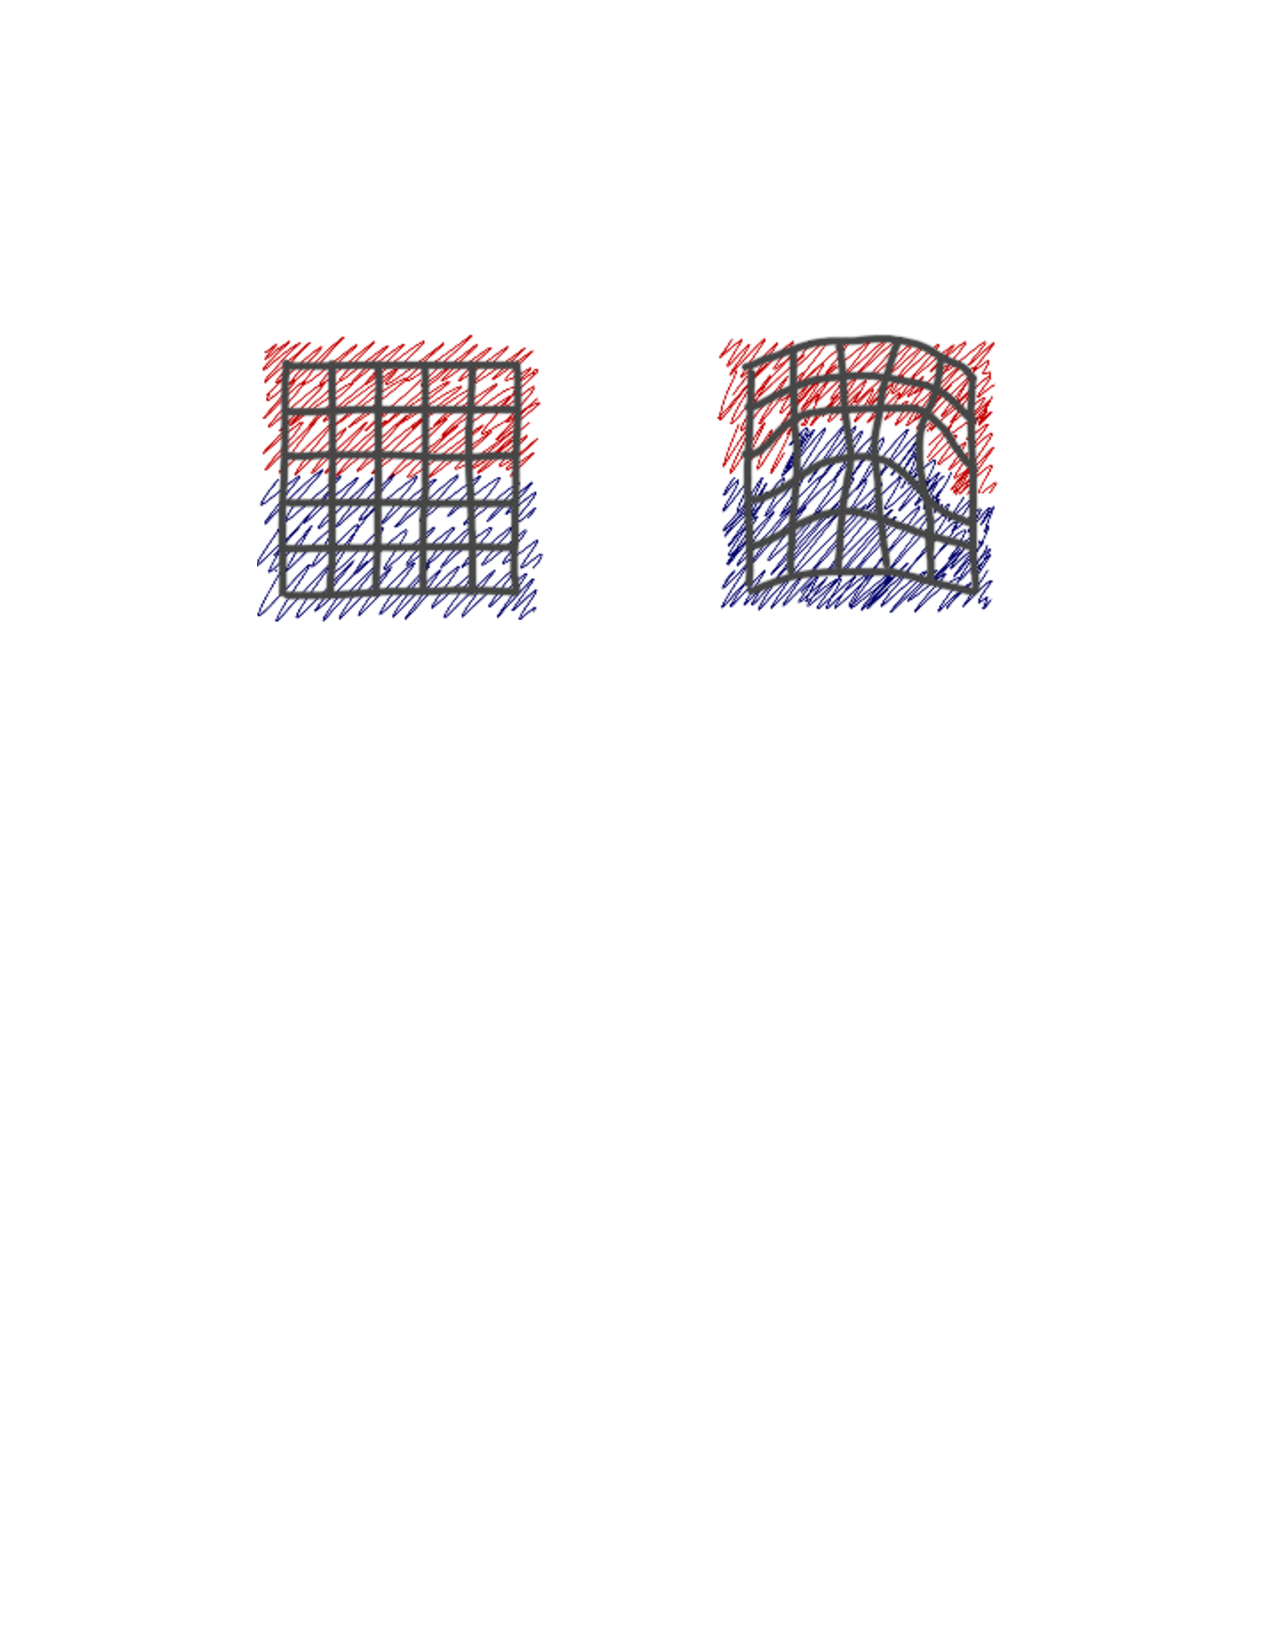
\includegraphics[width=\linewidth]{lagrangian}
\caption{\label{f.lagrangian-grid} A Lagrangian perturbation: we compare quantities for corresponding fluid elements.}
\end{marginfigure}

The two perturbations are related to one another via
\begin{equation}
\delta f = \Delta f + (\delta\vr\vdot\grad)f_{0}.
\end{equation}
There are a few useful commutation relations that are easily proved:
\begin{eqnarray}
\partial_{t}\Delta f &=& \Delta\left(\partial_{t}f\right),\\
\grad \Delta f &=& \Delta \grad f,\\
\frac{\Dif}{\Dif t}\delta f &=& \delta \frac{\Dif f}{\Dif t}.
\end{eqnarray}
And there are operations that do not commute:
\begin{eqnarray}
\partial_{t}\delta f &\neq& \delta\left(\partial_{t}f\right),\\
\grad \delta f &\neq& \delta \grad f,\\
\frac{\Dif}{\Dif t}\Delta f &\neq& \Delta \frac{\Dif f}{\Dif t}.
\end{eqnarray}
One can further show that $\delta\vu = (\Dif/\Dif t)\delta \vr$. Also, if the fluid has unperturbed velocity $\vu = 0$, then $\Delta \vu = \delta \vu$.  Finally, for purely radial motion, we can introduce the Lagrangian mass coordinate $m$, in which case $\partial_{m}\delta f = \delta(\partial_{m}f)$ and $\partial_{m}\Delta f \neq \Delta(\partial_{m}f)$.

\newthought{We are now ready to use these commutation relations to derive} a \emph{linear adiabatic wave equation}. By linear, we mean that we shall only keep terms to first order in $\delta$.  By adiabatic, we mean that we shall only consider the equations of continuity and momentum, and we shall relate the density and pressure perturbations via
\begin{equation}\label{e.adiabatic-condition}
 \frac{\delta P}{P} = \Gamma_{1}\frac{\delta \rho}{\rho}.
\end{equation}
Here $\Gamma_{1}\equiv \left(\partial\ln P/\partial\ln\rho\right)_{s}$.

For simplicity, we'll start with purely radial oscillations.
First, let's perturb the equation of continuity, expressed in Lagrangian form (eq.~[\ref{e.lagrange-r}]),
\[
\frac{\partial\ln r}{\partial m} = \frac{1}{4\pi r^{3}\rho}.
\]
We apply a Lagrangian perturbation to both sides of this equations and expand the right-hand side to first order in $\delta r$ and $\delta \rho$.  Since $\delta$ and $\partial/\partial_{m}$ commute, we can interchange them:
\begin{eqnarray*}
\frac{\partial}{\partial m}\left(\frac{\delta r}{r}\right) &=& \delta\left(\frac{\partial \ln r}{\partial m}\right)\\
	&=& \delta\left( 4\pi r^{3}\rho\right)^{-1} \\
	&=& \left(4\pi r^{3}\rho\right)^{-1}\left(-3 \frac{\delta r}{r} - \frac{\delta\rho}{\rho}\right).
\end{eqnarray*}
Moving $(4\pi r^{3}\rho)$ to the left-hand side of the equation, and recognizing that
\[ 4\pi r^{3}\rho \frac{\partial}{\partial m} = r\frac{\partial m}{\partial r}\frac{\partial }{\partial m} = r\frac{\partial }{\partial r}, \]
we have our first equation,
\begin{equation}\label{e.linearized-radial-continuity}
r\frac{\partial}{\partial r}\left(\frac{\delta r}{r}\right) = -3\frac{\delta r}{r} - \frac{\delta \rho}{\rho}.
\end{equation}
Next, we can perturb the force equation (eq.~[\ref{e.lagrange-momentum}])
\[
\frac{\Dif^{2} r}{\Dif t^{2}} = -\frac{Gm}{ r^{2}} - 4\pi r^{2}\frac{\partial P}{\partial m}.
\]
If the unperturbed state is taken to have $\Dif r_{0}/\Dif t = \Dif^{2} r_{0}/\Dif t^{2} = 0$, then a similar linearization yields
\begin{equation}\label{e.linearized-radial-momentum}
\rho r \frac{\Dif^{2} }{\Dif t^{2}}\left(\frac{\delta r}{r}\right) = -\frac{\partial P}{\partial r}\left(4\frac{\delta r}{r} + \frac{\delta P}{P}\right) - P \frac{\partial}{\partial r}\left(\frac{\delta P}{P}\right),
\end{equation}
which is our second equation.

To proceed further, we write
\[ \frac{\delta r}{r} = \zeta(r) \exp(i\sigma t), \]
so that the left-hand side of equation~(\ref{e.linearized-radial-momentum}) becomes $-\rho r \sigma^{2}\zeta(r) e^{i\sigma t}$, and we can make the substitution $\partial_{r} (\delta r/r) \to e^{i\sigma t}(\dif \zeta/\dif r)$.  We additionally eliminate $\delta \rho/\rho$ from equation~(\ref{e.linearized-radial-continuity}) using the adiabatic condition, eq.~(\ref{e.adiabatic-condition}) and make use of the zeroth-order momentum equation $\dif P/\dif r = -\rho Gm/r^{2}$ to obtain
\begin{eqnarray}
\label{e.linearized-one}
\frac{\dif}{\dif r}\zeta &=& -\frac{1}{r}\left(3\zeta + \frac{1}{\Gamma_{1}}\frac{\delta P}{P}\right)\\
\label{e.linearized-two}
\frac{\dif}{\dif r}\left(\frac{\delta P}{P}\right) &=& \frac{1}{\lambda_{P}}\left[\left( 4+ \sigma^{2}\frac{r^{3}}{Gm}\right)\zeta + \frac{\delta P}{P}\right].
\end{eqnarray}
Here we introduce the pressure scale height (in the unperturbed system) $\lambda_{P} \equiv -(\dif \ln P/\dif r)^{-1} = P r^{2}/(\rho Gm)$.  Multiply equation~(\ref{e.linearized-one}) by $\Gamma_{1} P r^{4}$ and then differentiate with respect to $r$, using equation~(\ref{e.linearized-two}) to eliminate the spatial derivative of $\delta P/P$ and equation~(\ref{e.linearized-one}) to eliminate $\delta P/P$ to obtain
\begin{equation}\label{e.LAWE}
\frac{\dif}{\dif r}\left[ \Gamma_{1}P r^{4} \frac{\dif}{\dif r}\zeta\right] + \left\{ r^{3}\frac{\dif}{\dif r}\left[\left( 3\Gamma_{1}-4\right)P\right]\right\} \zeta + \sigma^{2} (r^{4}\rho) \zeta = 0.
\end{equation}
Notice here that we have \emph{not} assumed that $\Gamma_{1}$ is a constant.

Equation~(\ref{e.LAWE}) has the form
\[
\mathcal{L}\zeta(r) + \sigma^{2} w(r) \zeta(r)
\]
where
\[
\mathcal{L} \equiv \frac{\dif}{\dif r}\left[ u(r) \frac{\dif \zeta}{\dif r}\right] + q(r)\zeta(r),
\]
with $u(r) = \Gamma_{1} P r^{4}$,
\[ q(r) = r^{3}\frac{\dif}{\dif r}\left[\left( 3\Gamma_{1}-4\right)P\right], \]
and $w(r) = r^{4}\rho$.  For the imposed boundary conditions, there will in general be solutions for only certain eigenvalues $\sigma^{2}$.  Note that $u(r) > 0$ on the interval $0 < r < R$.  Furthermore, we require that $\zeta$ and $\dif \zeta/\dif r$ be finite at $r = 0$ and $r = R$, which means that if $\zeta_{i}$ and $\zeta_{j}$ are solutions of eq.~(\ref{e.LAWE}), then
\begin{equation}\label{e.LAWE-boundary}
\left . u(r) \zeta_{i}^{*}\frac{\dif\zeta_{j}}{\dif r} \right |_{r = 0} = \left . u(r) \zeta_{i}^{*}\frac{\dif\zeta_{j}}{\dif r} \right |_{r = R} = 0.
\end{equation}
Using these boundary conditions and the form of the operator $\mathcal{L}$, we find that
\begin{eqnarray*}
 \int_{0}^{R}\dif r\; \zeta_{i}^{*} \mathcal{L}\zeta_{j} &=&  \left. u\zeta_{i}^{*}\frac{\dif\zeta_{j}}{\dif r}\right|_{r=0}^{r=R} -  \int_{0}^{R}\dif r\; \frac{\dif\zeta_{i}^{*}}{\dif r} u \frac{\dif\zeta_{j}}{\dif r} + \zeta_{j}q(r)\zeta_{i}^{*}\\
  &=& -\left. u(r) \zeta_{j}\frac{\dif\zeta_{i}^{*}}{\dif r} \right|_{r=0}^{r=R} + \int_{0}^{R}\dif r\; \zeta_{j}\frac{\dif}{\dif r}\left[u\frac{\dif}{\dif r}\zeta_{i}^{*}\right] + \zeta_{j}q(r)\zeta_{i}^{*} \\
   &=& \int_{0}^{R}\dif r\; \zeta_{j}\mathcal{L}\zeta_{i}^{*}.
 \end{eqnarray*}
The operator $\mathcal{L}$ is thus Hermitian.  As a result, the eigenvalues $\sigma^{2}$ are real and denumerable.  There is a minimum eigenvalue $\sigma^{2}_{0}$.  The eigenfunctions corresponding to these eigenvalues are orthogonal in the following sense: if $\sigma^{2}_{i}$ and $\sigma_{j}^{2}$ are eigenvalues of equation~(\ref{e.LAWE}) and $\zeta_{1}$, $\zeta_{2}$ their corresponding eigenfuctions, then
\begin{equation}\label{e.LAWE-orthogonality}
\int_{0}^{R}\dif r\; w(r) \zeta_{i}\zeta_{j} = \int_{0}^{R} \dif r\; r^{4}\rho \zeta_{i}\zeta_{j} = 0\quad \textrm{if} \;\sigma_{i}^{2} \neq \sigma_{j}^{2}.
\end{equation}
Solutions with larger eigenvalues have more nodes.

\section{Adiabatic non-radial pulsations}\label{s.adiabatic-non-radial}
Now that we've warmed up with the purely radial pulsations, we'll do the more general case.  Rather than going through the separation of variables in spherical coordinates, we'll keep things simple and cartesian.  This amounts to looking at a small box in the star.  We will also make an \emph{ansatz} that the fluid perturbations don't change the gravitational potential\sidenote{This is known as the \textbf{Cowling approximation}.}.  In this case, the (constant) gravitational acceleration $\vg = -g\bvec{e}_{r}$ defines the local vertical, so we will separate our equations into a radial direction, labeled by ``$r$'', and a transverse direction, labeled by ``$t$''.

Let us first perturb the equation of continuity,
\begin{equation}\label{e.continutiy-redux}
 \frac{\partial\rho}{\partial t} + \divr(\rho \vu) = \frac{\Dif\rho}{\Dif t} + \rho\divr\vu =  0.
\end{equation} 
We take our unpertubed state to be independent of time with $\vu = \bvec{0}$. If we take the Lagrangian perturbation of eq.~(\ref{e.continutiy-redux}), we have
\[ \frac{\Dif}{\Dif t}\left(\delta\rho + \rho\divr\vxi\right) = 0, \]
with $\vu = \Dif\vxi/\Dif t$.  Setting the constant of integration to $0$ reduces this to 
\[ \frac{\delta\rho}{\rho} = -\divr\vxi. \]
The linearization of the momentum equation,
\begin{equation}\label{e.momentum-redux}
 \frac{\Dif^{2} \vxi}{\Dif t^{2}} = - \frac{1}{\rho}\grad\Delta P + \frac{\Delta \rho}{\rho}\vg,
\end{equation}
looks very similar to what we did in deriving a condition for convection, \S~\ref{s.convection-second-look}. This time, however, we won't impose the condition that $\Delta P = 0$. When we were looking at convective instabilities, we were interested in low-frequency perturbations, in which the pressure has time to equilibrate.  Keeping the terms with $\Delta P$, the perturbed momentum equation becomes
\begin{equation}\label{e.perturbed-momentum-2}
\frac{\Dif^{2}\vxi}{\Dif t^{2}} = - \frac{1}{\rho}\grad\Delta P +  
\vg \underbrace{\frac{1}{\Gamma_{1}}\frac{\Delta P}{P} + \vg(\vxi\vdot\grad)
 \overbrace{\left[\frac{1}{\Gamma_{1}}\ln P-\ln \rho\right]}^{-\mathcal{A}}}_{\textrm{buoyancy from density perturbation}}.
\end{equation}
If $\Delta P\to 0$, this reduces to equation~(\ref{e.blob-eq-of-motion}) with $\mathcal{A}$ being the \textbf{Schwarzschild discriminant}.


To decompose our perturbed system into normal modes, with the perturbed quantities varying in time as $\exp(i\omega t)$, we first note that
in the unperturbed system $\ln P$ and $\ln\rho$ depend only on $r$; and nothing depends on the transverse directions.  As a result, we can impose periodic boundary conditions in the transverse direction  and write
\begin{eqnarray*}
\Delta P(\vx,t) &=& \Delta P(r) \exp(i\vkt\vdot \vx_{t})\exp(i\omega t),\\
\Delta \vxi(\vx,t) &=& \vxi(r) \exp(i\vkt\vdot \vx_{t})\exp(i\omega t).
\end{eqnarray*}
Here $\vkt$ is a transverse wavenumber and $\vx_{t}$ are the transverse coordinates.
The transverse component of equation~(\ref{e.perturbed-momentum-2}) is thus
\begin{equation}\label{e.transverse-perturbed-momentum}
\rho\omega^{2} \vxi_{t} = i \vkt \Delta P,
\end{equation}
and the radial equation of motion is
\begin{equation}\label{e.radial-perturbed-momentum}
\rho\omega^{2}\xi_{r} = \partial_{r}\Delta P + \frac{g\rho}{\Gamma_{1}P}\Delta P  + \rho N^{2} \xi_{r}.
\end{equation}
We've re-introduced the Brunt-V\"ais\"al\"a frequency\sidenote{We take $\Gamma_{1}$ to be constant.}
\[ N^{2} = -g\frac{\dif}{\dif r}\mathcal{A} = g\left(\frac{1}{\Gamma_{1}}\frac{\dif}{\dif r}\ln P - \frac{\dif}{\dif r}\ln \rho\right), \]
just as was done in analyzing convection.

We still have more unknowns than equations.  Next, we'll use the perturbed equation of continuity, 
\begin{equation}\label{e.perturbed-continuity}
\frac{\delta\rho}{\rho} = -\divr\vxi = -\partial_{r}\xi_{r} - \vkt\vdot\vxi_{t}.
\end{equation}
For adiabatic perturbations,
\begin{eqnarray*}
\frac{\delta\rho}{\rho} &=& \frac{1}{\Gamma_{1}}\frac{\delta P}{P}\\ 
	&=& \frac{1}{\Gamma_{1}}\left(\frac{\Delta P}{P} + \vxi\vdot\grad\ln P\right)\\
		&=& \frac{1}{\Gamma_{1}}\frac{\Delta P}{P} - \xi_{r}\frac{1}{\Gamma_{1} \lambda_{P}}.
\end{eqnarray*}
Here we used $\vxi\vdot\grad \ln P = \xi_{r}(\dif/\dif r) \ln P = -\xi_{r}\rho g/P = -\xi_{r}/\lambda_{P}$, where $\lambda_{P}$ is the pressure scale height.  It makes physical sense that this scale will enter: modes with radial wavelengths much less than $H$ shouldn't be affected by the background stratification.

Inserting the expression for $\delta\rho/\rho$ in equation~(\ref{e.perturbed-continuity}) and  using equation~(\ref{e.transverse-perturbed-momentum}) to eliminate $\vxi_{t}$, we obtain
\begin{equation}\label{e.radial-lamb}
\partial_{r} \xi_{r} = \frac{1}{\omega^{2}\Gamma_{1}P} \left(\frac{k_{t}^{2}\Gamma_{1}P}{\rho} - \omega^{2}\right)\Delta P + \frac{\xi_{r}}{\Gamma_{1}\lambda_{P}}.
\end{equation}
The quantity $S^{2} = k_{t}^{2} \Gamma_{1}P/\rho = k_{t}^{2}c_{s}^{2}$ is called the \textbf{Lamb frequency}.

Collecting equations~(\ref{e.radial-lamb}) and (\ref{e.radial-perturbed-momentum}), we now have two coupled first order differential equations for $\xi_{r}(r)$ and $\Delta P(r)$,
\begin{eqnarray}
\label{e.normal-mode-1}
\partial_{r}\xi_{r} &=& \frac{1}{\Gamma_{1}P} \frac{S^{2}-\omega^{2}}{\omega^{2}}\Delta P + \frac{\xi_{r}}{\Gamma_{1}\lambda_{P}}\\
\label{e.normal-mode-2}
\partial_{r}\Delta P &=& \rho(\omega^{2}-N^{2})\xi_{r} - \frac{\Delta P}{\Gamma_{1}\lambda_{P}}.
\end{eqnarray}
From the form of these equations, let's try a solution in the form
\begin{equation}\label{e.trial-radial-solution}
	\Delta P(r) = \Delta P e^{Kr}; \qquad \xi_{r}(r) = \xi_{r}e^{Kr}.
\end{equation}
If $K$ is imaginary, then we have oscillatory solutions.  If $K$ is real, then we must choose $K$ so that the radial functions decay exponentially, or \textbf{evanesce}.  Substituting equation~(\ref{e.trial-radial-solution}) into eq.~(\ref{e.normal-mode-2}) gives
\[
\Delta P = \left[\frac{\rho(\omega^{2}-N^{2})}{1 + 1/K\lambda_{P}}\right] \frac{\xi_{r}}{K}.
\]
Substituting this expression for $\Delta P$ into eq.~(\ref{e.normal-mode-1}) and eliminating $\xi_{r}$ gives us the dispersion equation,
\begin{equation}\label{e.full-dispersion-equation}
K^{2} = \frac{k_{t}^{2}}{S^{2}} \frac{(S^{2} - \omega^{2})(\omega^{2}-N^{2})}{(1 + 1/K\lambda_{P})\omega^{2}} + \frac{1}{K\lambda_{P}},
\end{equation}
which relates the mode frequency $\omega$ to the transverse wavenumber $k_{t}$ and the radial wavenumber $K$.

In the limit where the radial wavelength is much less than a pressure scale height, $|K|\lambda_{P}\gg 1$, equation~(\ref{e.full-dispersion-equation}) simplifies to
\begin{equation}\label{e.dispersion-equation}
K^{2} = \frac{k_{t}^{2}(S^{2} - \omega^{2})(\omega^{2}-N^{2})}{S^{2}\omega^{2}}.
\end{equation}
If $N^{2} < \omega^{2} < S^{2}$, $K^{2} > 0$ and the radial perturbations evanesce.  To have a mode, we require either that $\omega^{2} < N^{2}, S^{2}$ or $\omega^{2} > N^{2}, S^{2}$.  

The analysis is similar in spherical coordinates, except that instead of plane waves, $e^{\vkt\vdot\vx_{t}}$, we'll have spherical harmonics $Y_{\ell m}$.  In the above dispersion relation, make the substitution $k_{t}^{2} \to \ell(\ell + 1)/r^{2}$ and $S^{2} \to S^{2}_{\ell}$.

\begin{exercisebox}
Use dimensional analysis and virial estimates to sketch $S$ (for $\ell = 1$) and $N$ on a plot of frequency against radius for the sun. Indicate where modes with $\omega^{2} < N^{2}, S^{2}$ can propagate, and likewise for $\omega^{2} > N^{2}, S^{2}$.
\end{exercisebox}
